\section{Goods per Agent}\label{sec:goods}
%% FUNCTION: Shows how the EFX rate of round robin changes with the number of goods per agent r
%% when the number of goods is divisible by the number of agents (q = 0; m = 8, 12, 16 for n = 4).
%% More goods per agent help unless agents agree strongly. Special case: if every agent receives
%% at most two goods and all favourite goods differ, round robin is guaranteed to be EFX (proven);
%% the guarantee breaks at m = 2n + 1. Since this break coincides with the first remainder, the
%% section leads to divisibility.

Return to the father and his four children, but suppose that his collection holds $8$, $12$ or
$16$ records. Each child then picks two, three or four times. More picks give the children who
pick late more chances to catch up, but they also give everyone more records to envy in a
sibling's allocation. In our notation, the number of picks per child is the number of full rounds
$r$. To keep divisibility out of this comparison, the number of records is always a multiple of
four. Agreement and dispersion stay at $\rho=0.5$ and
$\theta=1$, so that $r=3$ is the reference cell. With a single record per child, the collection
would be no larger than the family, a case we exclude (Section~\ref{sec:setting}), so the
comparison starts at $r=2$.

\subsection{EFX Rate}\label{sec:goods-rate}

As Figure~\ref{fig:goods} shows, Round Robin achieves EFX more often when every agent receives
more goods. With two goods per agent, the EFX rate is $0.212$, with $15{,}755$ failures among
$R=20{,}000$ instances. It rises to $0.293$ with three goods and to $0.409$ with four goods, where
$11{,}828$ instances fail.

\begin{figure}[H]
  \centering
  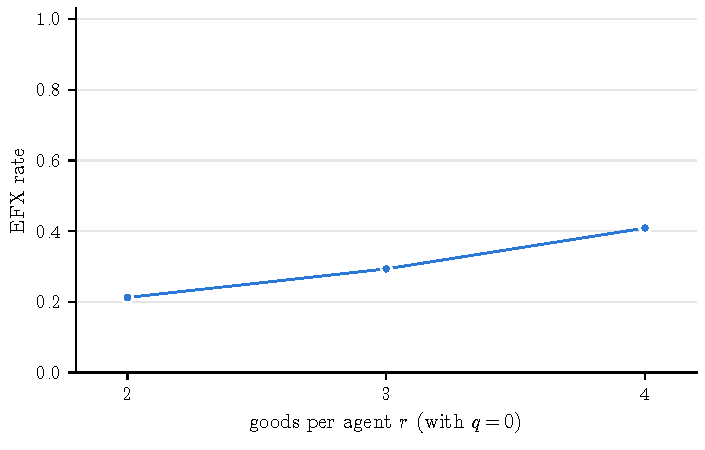
\includegraphics{fig43_goods_rate.pdf}
  \caption{EFX rate of Round Robin against the number of goods per agent $r$, for $n=4$ agents
  with $m=4r$ goods ($q=0$), agreement $\rho=0.5$ and dispersion $\theta=1$. Each point rests on
  $R=20{,}000$ instances. The line between the points is for illustration only.}
  \label{fig:goods}
\end{figure}

The same trend holds for the other cells of our design: the EFX rate almost always rises with
every additional full round, or is already $1$. The exception is a world in which all agents rank
the goods identically, where additional rounds do not help. Apart from this case, the more goods
each person receives, the more likely Round Robin is to achieve EFX.

\subsection{At Most Two Goods and Distinct Favourite Goods}\label{sec:bundlesize}

With few goods per agent, there is a case in which Round Robin is guaranteed to achieve EFX. It
depends on whether the agents have different favourite goods. We call an instance
\textit{collision-free} if all agents have different favourite goods. Under full agreement
($\rho=1$), all agents have the same favourite good, so no instance is collision-free.

\begin{lemma}\label{lem:bundlesize}
Suppose that all agents have different favourite goods. Then under Round Robin, no agent violates
EFX towards an agent who receives at most two goods.
\end{lemma}

\begin{proof}
Let $i$ and $j$ be two agents with $|A_j|\leq2$. Since all favourite goods differ, every agent
receives their favourite good in the first round, so $v_i(A_i)\geq v_i(g)$ for every good $g$. If
$|A_j|=1$, EFX holds trivially for this pair. If $|A_j|=2$, removing either good from $A_j$ leaves
a single good $g$, and $v_i(g)\leq v_i(A_i)$.
\end{proof}

\begin{corollary}\label{cor:bundlesize}
If an instance is collision-free and $m\leq2n$, the Round Robin allocation is EFX.
\end{corollary}

\begin{proof}
For $m\leq2n$, Round Robin gives every agent at most two goods, so Lemma~\ref{lem:bundlesize}
applies to every pair.
\end{proof}

The stored cells confirm the corollary: at every number of agents with $m\leq2n$, at every level
of agreement below $1$ and at every level of dispersion, each collision-free instance is EFX. The
proof uses only the favourite goods and the bundle sizes, so the guarantee does not depend on our
distribution of values. To our knowledge, it has not been stated explicitly before.

A related observation explains why the EFX rate at $m=n+1$ does not depend on dispersion
(Section~\ref{sec:dispersion-rate}). With one good more than agents, only one agent receives two
goods. For every other pair, EFX holds trivially or requires $v_i(A_i)\geq\max_{g\in A_j}v_i(g)$,
a comparison of single goods that depends only on the rankings. Since dispersion does not change
rankings, the EFX rate at $m=n+1$ is the same for every level of dispersion (proven; in the
stored cells it is identical instance by instance).

The condition of the corollary quickly becomes rare. Table~\ref{tab:collisionfree} shows the
share of collision-free instances at $m=2n$, the largest number of goods the guarantee covers. It
falls from $0.749$ for two agents without agreement to $0.010$ for five agents at $\rho=0.75$.

\begin{table}[H]
  \centering
  \caption{Share of collision-free instances at $m=2n$ goods, $R=20{,}000$ per cell. The share
  does not depend on dispersion.}
  \label{tab:collisionfree}
  \begin{tabular}{lcccc}
    \toprule
    $n$ & $\rho=0$ & $\rho=0.25$ & $\rho=0.5$ & $\rho=0.75$ \\
    \midrule
    2 & 0.749 & 0.650 & 0.535 & 0.379 \\
    3 & 0.553 & 0.398 & 0.256 & 0.126 \\
    4 & 0.405 & 0.231 & 0.115 & 0.038 \\
    5 & 0.299 & 0.140 & 0.051 & 0.010 \\
    \bottomrule
  \end{tabular}
\end{table}

Figure~\ref{fig:goods-break} shows what happens beyond $m=2n$ for four agents, restricted to
collision-free instances. Up to $m=8$, the EFX rate is exactly $1$, as the corollary states. As
soon as one agent receives a third good, it drops to $0.830$ at $m=9$, and by
Lemma~\ref{lem:bundlesize}, every violation is then towards the agent with three goods. The drop
does not come from the remainder: at $m=5$, $6$ and $7$, goods are left over as well, and the EFX
rate is still $1$. To the right of the break, the EFX rate recovers unevenly, to $0.941$ at
$m=16$.

\begin{figure}[H]
  \centering
  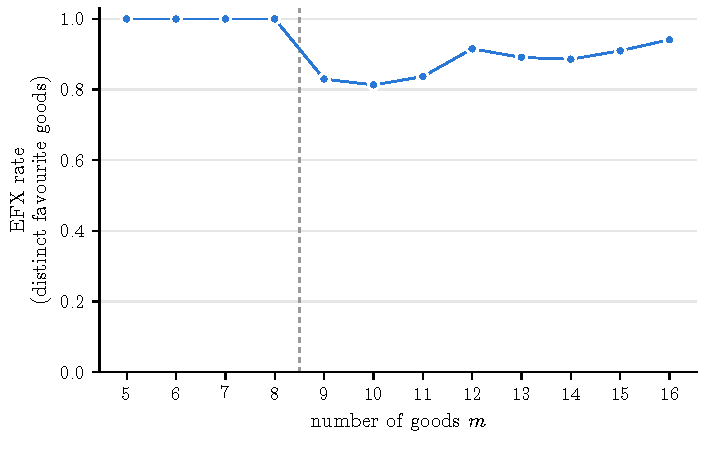
\includegraphics{fig43_goods_break.pdf}
  \caption{EFX rate of Round Robin among collision-free instances against the number of goods
  $m$, for $n=4$ agents, agreement $\rho=0.5$ and dispersion $\theta=1$. Left of the dashed line,
  no agent receives more than two goods. The number of collision-free instances per point ranges
  from $861$ at $m=5$ to $4{,}928$ at $m=16$ out of $R=20{,}000$. The line between the points is
  for illustration only.}
  \label{fig:goods-break}
\end{figure}

This does not contradict Section~\ref{sec:goods-rate}, because the guarantee covers only the
collision-free instances. Over all instances, the EFX rate still rises with the number of goods
per agent, from $0.212$ with two to $0.293$ with three (Figure~\ref{fig:goods}).

\subsection{Severity of Failures}\label{sec:goods-severity}

Figure~\ref{fig:goods-survival} shows the survival curves for two, three and four goods per
agent. A curve for more goods per agent never lies below a curve for fewer goods, so more rounds
reduce both the number and the depth of failures. At $\alpha=0.6$, the share of instances that
reach at least this level is $0.468$, $0.651$ and $0.787$. The conditional $5\%$ quantile rises
from $0.14$ to $0.23$ and $0.30$, and the median of $\astar$ among the instances that are not EFX
rises from $0.47$ to $0.60$ and $0.69$. Severe failures become rare: the share of instances with
$\astar<0.2$ falls from $0.090$ with two goods per agent to $0.024$ and $0.008$.

\begin{figure}[H]
  \centering
  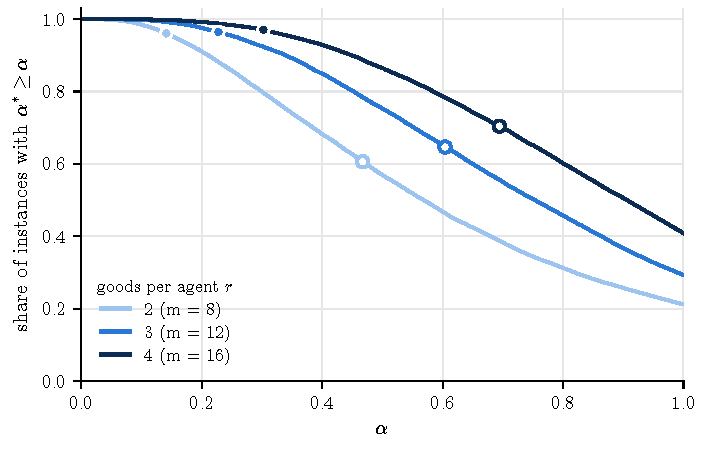
\includegraphics{fig43_goods_survival.pdf}
  \caption{Share of instances with $\astar\geq\alpha$ under Round Robin, one curve per number of
  goods per agent, for $n=4$ agents with $m=4r$ goods ($q=0$), Spearman $0.48$ ($\rho=0.5$) and
  Gini $0.52$ ($\theta=1$). Each curve rests on $R=20{,}000$ instances. The point on each curve
  marks the $5\%$ quantile of $\astar$ among the instances that are not EFX.}
  \label{fig:goods-survival}
\end{figure}

\paragraph{Relation to literature.}
Our results fit the asymptotic picture for independent values. \textcite[Thm.~3.1]{manurangsi2021}
show that Round Robin even achieves envy-freeness with high probability once the number of goods
is of order $n\log n/\log\log n$, for independent values whose density on $[0,1]$ is bounded.
Their result does not formally apply to our lognormal values, and it concerns many agents, but it
points in the same direction as our measurements at low agreement: more goods per agent help.
\textcite[p.~17]{manurangsi2021} also argue that standard Round Robin with one round and a large
remainder fails EFX with constant probability, because the last agent may lose their favourite
good to one of the agents who pick an extra good. This is the collision mechanism behind
Lemma~\ref{lem:bundlesize}, in asymptotic form. The existence of an EFX allocation is proven in
most cells with $m\leq2n$: for $n\leq3$ \parencite{plaut2020,chaudhury2024}, for $m\leq n+2$
\parencite{amanatidis2020multiple} and for $m\leq n+3$ \parencite{mahara2024general}. For $n=4$,
it is open from $m=8$ on, so all three cells of Figure~\ref{fig:goods} lie in the region where we
assume existence (Section~\ref{sec:existence}).

\paragraph{Recommendation.}
If every person receives at most two goods and all favourite goods differ, Round Robin delivers
EFX for certain, and both conditions can be checked before picking starts; beyond that, more goods
per person make EFX more likely, unless everyone agrees on what is valuable. Because the
guarantee breaks exactly where the first agent receives one good more than the others, the next
section asks what divisibility does.
